\documentclass[11pt,twoside,reqno]{amsart}
\usepackage{amssymb, amsmath, enumerate, palatino, hyperref}
\usepackage[normalem]{ulem}
%\usepackage{fullpage}
\usepackage[margin=1in]{geometry}
\usepackage[T1]{fontenc}
\renewcommand{\labelitemi}{\guillemotright}
\usepackage{mathrsfs}
%--------------------------------
% Kees' imports
%--------------------------------
\usepackage{physics}
\usepackage{tensor}
\usepackage{mathtools}
\usepackage{xcolor}
\usepackage{siunitx}
\usepackage{empheq}
\usepackage{tensor}


\theoremstyle{plain}
\newtheorem{prop}{Proposition}%[section]
\newtheorem{lemma}[prop]{Lemma}
\newtheorem{thm}[prop]{Theorem}
\newtheorem{obs}[prop]{Observation}
\newtheorem{app}[prop]{Application}
\newtheorem*{MainThm}{Main Theorem}
\newtheorem{cor}[prop]{Corollary}
\newtheorem{conj}[prop]{Conjecture}
\theoremstyle{remark}
\newtheorem{rmk}[prop]{Remark}
\theoremstyle{definition}
\newtheorem{prob}{Problem}
\newtheorem{bonus}[prop]{Bonus Problem}
\theoremstyle{remark}
\newtheorem{exc}{Exercise}
\newtheorem*{soln}{Solution}
\theoremstyle{definition}
\newtheorem{ex}[prop]{Example}
\theoremstyle{definition}
\newtheorem{defn}[prop]{Definition}

\newcommand{\RR}{\mathbb{R}}
\newcommand{\ZZ}{\mathbb{Z}}
\newcommand{\CC}{\mathbb{C}}
\newcommand{\NN}{\mathbb{N}}
\newcommand{\QQ}{\mathbb{Q}}

\newcommand{\Aut}{\operatorname{Aut}}

\newcommand{\defeq}{:=}

\renewcommand{\Re}{\operatorname{Re}}

%--------------------------------
% Kees' commands
%--------------------------------
\makeatletter
\newcommand{\subalign}[1]{%
  \vcenter{%
    \Let@ \restore@math@cr \default@tag
    \baselineskip\fontdimen10 \scriptfont\tw@
    \advance\baselineskip\fontdimen12 \scriptfont\tw@
    \lineskip\thr@@\fontdimen8 \scriptfont\thr@@
    \lineskiplimit\lineskip
    \ialign{\hfil$\m@th\scriptstyle##$&$\m@th\scriptstyle{}##$\hfil\crcr
      #1\crcr
    }%
  }%
}
\makeatother

\newcommand{\allspace}{{\substack{\text{all}\\\text{space}}}}

\newcommand{\DD}{\mathbb{D}}
\renewcommand{\AA}{\mathbb{A}}
\newcommand{\VV}{\mathbb{V}}
\newcommand{\LL}{\mathbb{L}}
\newcommand{\BB}{\mathbb{B}}
\renewcommand{\SS}{\mathbb{S}}
\newcommand{\HH}{\mathbb{H}}

\renewcommand{\l}{\ell}

\newcommand{\PB}{\mathrm{PB}}

\newcommand{\cL}{\mathcal{L}}
\newcommand{\cE}{\mathcal{E}}
\newcommand{\cH}{\mathcal{H}}
\newcommand{\cC}{\mathcal{C}}
\newcommand{\cA}{\mathcal{A}}
\newcommand{\cI}{\mathcal{I}}
\newcommand{\cM}{\mathcal{M}}
\newcommand{\cO}{\mathcal{O}}

\newcommand{\sgn}{\mathrm{sgn}}

\newcommand{\LIPS}{\mathrm{LIPS}}
\newcommand{\zcut}{z_\mathrm{cut}}
\newcommand{\mMDT}{\mathrm{mMDT}}

\newcommand{\Ei}{\mathrm{Ei}}
\newcommand{\Li}{\mathrm{Li}}

\newcommand{\arctanh}{\mathrm{arctanh}}
\newcommand{\arcsinh}{\mathrm{arcsinh}}

\newcommand{\nc}{\mathrm{nc}}
\newcommand{\cusp}{\mathrm{cusp}}

\def\beq#1\eeq{\begin{equation}#1\end{equation}}
\def\bal#1\eal{\begin{align}#1\end{align}}

\title{Calculating the soft function}
\author{Kees Benkendorfer}
\date{24 February 2021}

\begin{document}
\maketitle

\tableofcontents

\section{Setup}
	We wish to calculate the resolved soft function $S_R(\rho - \zcut)$ which describes soft radiation which passes the groomer due to proximity to the resolved gluon. If the resolved emission occurs at an angle $\theta$ from the quark axis, then any radiation at smaller angles will pass the groomer. A schematic of this situation is displayed in Fig.~\ref{fig:schematic}.

	The goal is to calculate the first-order term in an expansion of $S_R$. We can then use renormalization group evolution in conjunction with the other first-order results of functions in the factorization equation to achieve an all-orders calculation of the cross section.

	Let the resolved gluon have momentum $k_g$, the quark lie along direction $n_q = (1, 0, 0, 1)$, and consider an extra-soft gluon with momentum $k$. If the extra-soft gluon is closer to the quark, then its dominant contribution to the jet mass $\rho$ will come from its interaction with the quark:
	\begin{equation}
		\rho = \frac{4 k^+}{Q}
	\end{equation}
	where $k^{\pm} = k^0 \mp k_z$ are light-cone coordinates defined with respect to the quark axis. If the extra-soft gluon is closer to the resolved gluon, then its contribution to the jet mass from the quark interaction has already been accounted for in the contribution of the resolved gluon. The leading-order contribution from the new gluon therefore comes with its interaction with the resolved gluon. If $n_g$ is the direction of the resolved gluon, then the contribution is
	\begin{equation}
		\rho = \frac{4 k \cdot n_g}{Q} = \frac{4 k \cdot k_g}{E_g Q}
	\end{equation}
	with $E_g$ the energy of the resolved gluon.

	Notice that the angle between the extra-soft gluon and the quark is given by
	\begin{equation}
		1 - \cos\theta_{gq} = \frac{k^+}{k^0}
	\end{equation}
	while the angle between the extra-soft gluon and the resolved gluon is
	\begin{equation}
		1 - \cos\theta_{gg} = \frac{k \cdot n_g}{k^0}.
	\end{equation}
	The case in which the extra-soft gluon is closer to the quark is the case in which $\theta_{gq} < \theta_{gg}$, so $1 - \cos\theta_{gq} < 1 - \cos\theta_{gg}$ and, in turn $k^+ < k \cdot n_g$. Therefore, the total measurement function is
	\begin{equation}
		\delta_\rho = \Theta(k\cdot n_g - k^+)\,\delta\qty(\rho - \frac{4k^+}{Q}) + \Theta(k^+ - k\cdot n_g)\,\delta\qty(\rho - \frac{4k\cdot n_g}{Q}).
	\end{equation}

	\begin{figure}\label{fig:schematic}
		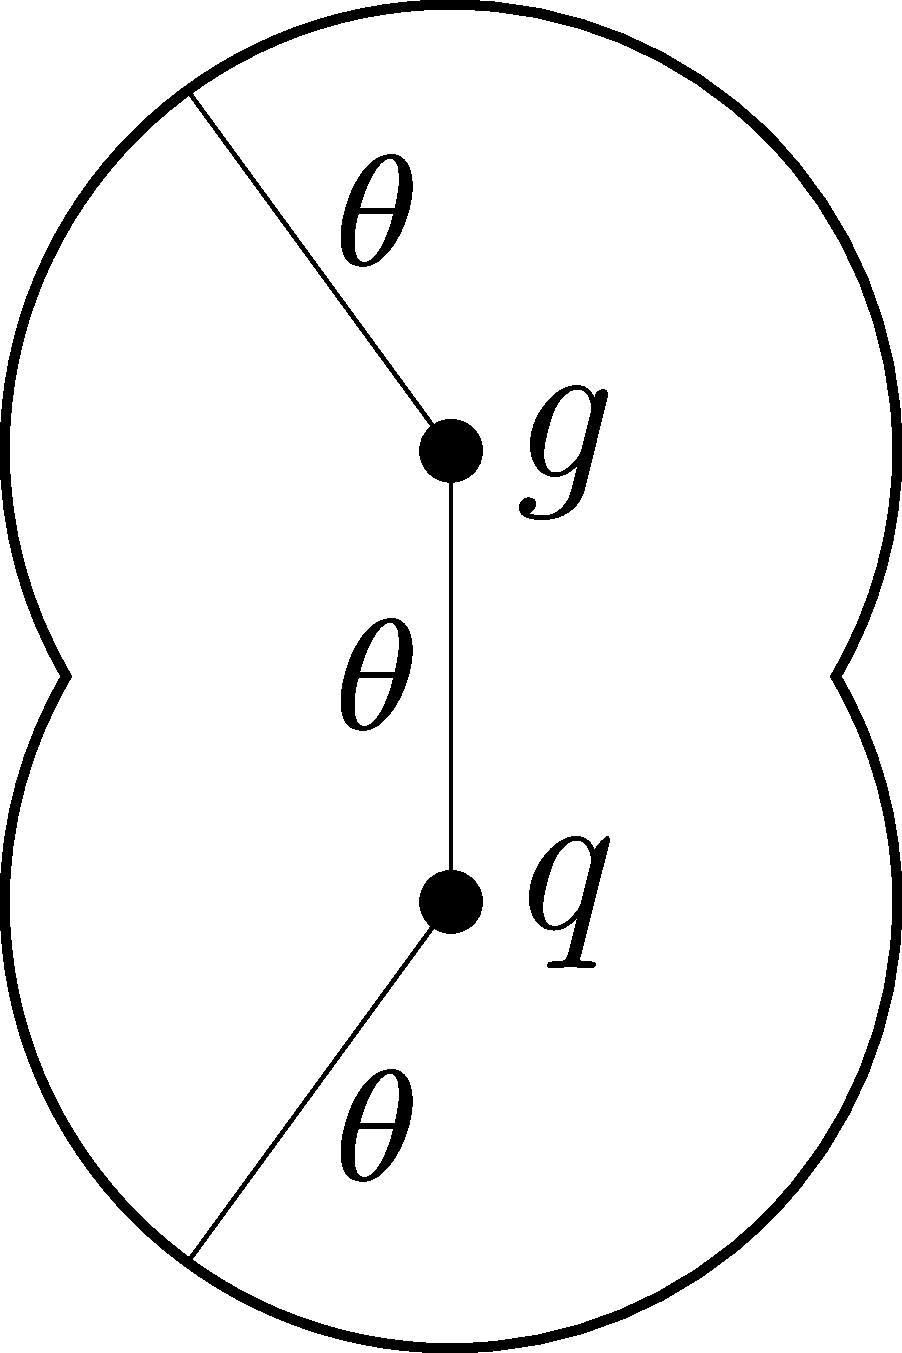
\includegraphics[width=0.15\textwidth]{figures/head_on_schematic.pdf}
		\caption{Schematic head-on view of emissions according to the jet groomer. Radiation within the peanut-shaped region will pass the grooming algorithm.}
	\end{figure}

	We also need to impose the kinematic constraint that the gluon is in the peanut-shaped region of Fig.~\ref{fig:schematic}. Saying that the gluon is in the region is equivalent to saying that it is not outside the region. The gluon is outside of the quark's radius of influence if
	\begin{equation}
		\frac{k^+}{k^0} = 1 - \cos\theta_{gq} > 1 - \cos\theta = n_g \cdot n_q.
	\end{equation}
	On the other hand, the gluon is outside the resolved gluon's radius of influence if
	\begin{equation}
		\frac{k \cdot n_g}{k^0} = 1 - \cos\theta_{gg} > 1 - \cos\theta = n_g \cdot n_q.
	\end{equation}
	Therefore, the grooming restriction is
	\begin{equation}
		\Theta_{\mMDT} = 1 - \Theta(k^+ - k^0 n_g \cdot n_q)\,\Theta(k \cdot n_g - k^0 n_g \cdot n_q).
	\end{equation}

	The matrix element accounts for the possibility that the gluon be emitted from any pairs of resolved particles {\color{red}\textbf{[TODO: it's not actually a sum]}} \cite{catani_infrared_2000}
	\begin{equation}\label{eq:matrix element general}
		\abs{\cM}^2 = -\mu^{2\epsilon}\sum_{i < j} \vb{T}_i \cdot \vb{T}_j \frac{n_i \cdot n_j}{(n_i \cdot k)(n_j \cdot k)}
	\end{equation}
	where $i, j$ range over all pairs of resolved particles and the $\vb{T}_i$ are color matrices. Each term of the matrix element corresponds to a separate soft function. For now, we will focus on the first term \cite{catani_infrared_2000}
	\begin{equation}
		\abs{\cM_{q\bar q}}^2 = -4\pi\alpha_s C_F \mu^{2\epsilon}\frac{n_q \cdot n_{\bar q}}{(n_q \cdot k)(n_{\bar q}\cdot k)} = -4\pi\alpha_s C_F \mu^{2\epsilon}\frac{2}{k^+ k^-}
	\end{equation}
	with $n_{\bar q} = (1, 0, 0, -1)$ the antiquark direction. {\color{red}\textbf{[TODO: need to handle other soft functions}}

	Finally, phase space in $d$ dimensions takes the usual form
	\begin{equation}
		d\Pi = \frac{d^d k}{(2\pi)^d} 2\pi\,\delta\qty(k^2)\,\Theta(k^+)\,\Theta(k^- - k^+).
	\end{equation}
	Notice that we are enforcing the gluon to be emitted in the hemisphere with the quark by requiring $k^- - k^+$. We will multiply the result at the end by a factor of $2$ to account for the case where the gluons are emitted in the other hemisphere. Note that we are only scanning over the momentum of the extra-soft gluon: under the assumption that this gluon is softer than the resolved gluon, this emission does not influence the momentum of the quarks or resolved gluon.

	Putting everything together, we find
	\begin{equation}\label{eq:soft integral}
	\begin{aligned}
		S_R(\rho - \zcut) = -8\pi\alpha_s C_F \mu^{2\epsilon} \int& \frac{d^d k}{(2\pi)^{d-1}} \, \delta\qty(k^2)\,\Theta(k^+)\,\Theta(k^- - k^+) \,\frac{2}{k^+ k^-} \\
		&\times \qty[\Theta(k\cdot n_g - k^+)\,\delta\qty(\rho - \frac{4k^+}{Q}) + \Theta(k^+ - k\cdot n_g)\,\delta\qty(\rho - \frac{4k\cdot n_g}{Q})] \\
		&\times \qty[1 - \Theta(k^+ - k^0 n_g \cdot n_q)\,\Theta(k \cdot n_g - k^0 n_g \cdot n_q)].
	\end{aligned}
	\end{equation}

\section{Coordinate choice}
	Now we need to determine which coordinates in which to work. Notice that, physically, there is an axial symmetry to the problem: nothing depends on the angle of the resolved emission about the quark axis. Therefore, we might define our momenta in terms of their transverse momentum, pseudorapidity, and angle about the axis. To get from Cartesian $(p_x, p_y, p_z)$ to this detector coordinate system $(p_\perp, \phi, \eta)$, we use the following transformations:
	\begin{equation}
	\begin{aligned}
		p_x &= p_\perp \cos\phi & p_y &= p_\perp \sin\phi & p_z &= p_\perp \sinh\eta & p_0 &= p_\perp \cosh\eta \\
		p_\perp &= \sqrt{p_x^2 + p_y^2} & \phi &= \arctan(\frac{p_y}{p_x}) & \eta &= \arctanh\qty(\frac{p_z}{\abs{\vb{p}}}).
	\end{aligned}
	\end{equation}

	Under this transformation, the extra-soft gluon has momentum
	\begin{equation}
		k = (k_0, k_\perp, \phi_k, \eta_k).
	\end{equation}
	The resolved gluon is fixed in space from the perspective of the extra-soft gluon, so we can write it in whichever coordinates are convenient. Let us pick spherical coordinates, where the gluon momentum has an azimuthal angle $\phi_g$ and an angle $\theta_g$ from the jet axis
	\begin{equation}
		k_g = (k_0, r, \theta, \phi) = (E_g, E_g, \theta_g, \phi_g)
	\end{equation}
	and hence direction vector
	\begin{equation}
		n_g = \qty(1, 1, \theta_g, \phi_g).
	\end{equation}
	Finally, without loss of generality, we can define our coordinate axes so that the resolved emission is at angle $\phi_g = 0$, thereby setting
	\begin{equation}
	\begin{aligned}
		k_g &= (E_g, E_g, \theta_g, 0) & n_g &= (1, 1, \theta_g, 0).
	\end{aligned}
	\end{equation}

	Now we can transform each term of Eq.~\ref{eq:soft integral}. First, notice that
	\begin{equation}\label{eq:kplus coordinates}
		k^+ = k_0 - k_z = k_\perp \qty(\cosh\eta_k - \sinh\eta_k) = k_\perp e^{-\eta_k},
	\end{equation}
	and similarly
	\begin{equation}
		k^- = k_\perp e^{\eta_k}.
	\end{equation}
	Hence, the restriction $k^+ > 0$ becomes $k_\perp > 0$ and $k^- > k^+$ becomes $\eta_k > 0$. That is,
	\begin{equation}
		\Theta(k^+)\,\Theta(k^- - k^+) = \Theta(k_\perp)\,\Theta(\eta_k).
	\end{equation}
	The first term in the matrix element is then simply
	\begin{equation}
		\abs{\cM}^2 = -4\pi\alpha_sC_F\frac{2}{k^+ k^-} = -4\pi\alpha_sC_F\frac{2}{k_\perp^2}.
	\end{equation}

	Next comes the measurement function. First notice that (in Cartesian coordinates)
	\begin{equation}\label{eq:k dot ng coordinates}
	\begin{aligned}
		k \cdot n_g &= (k_\perp \cosh\eta_k, k_\perp \cos\phi_k, k_\perp \sin\phi_k, k_\perp\sinh\eta_k) \cdot (1, \sin\theta_g, 0, \cos\theta_g) \\
		&= k_\perp \qty[\cosh\eta_k - \cos\phi_k \sin\theta_g - \sinh\eta_k \cos\theta_g].
	\end{aligned}
	\end{equation}
	Therefore
	\begin{equation}
	\begin{aligned}
		\Theta(k^+ - k\cdot n_g) &= \Theta\qty(\cos\phi_k \sin\theta_g - (1- \cos\theta_g)\sinh\eta_k) \\
		&= \Theta\qty(\cos\phi_k\frac{\sin\theta_g}{1 - \cos\theta_g} - \sinh\eta_k) \\
		&= \Theta\qty(\cos\phi_k\cot\frac{\theta_g}{2} - \sinh\eta_k)
	\end{aligned}
	\end{equation}
	and
	\begin{equation}
		\Theta(k\cdot n_g - k^+) = \Theta\qty(\sinh\eta_k - \cos\phi_k\cot\frac{\theta_g}{2}).
	\end{equation}
	The full measurement function is then
	\begin{equation}
	\begin{aligned}
		\delta_\rho &= \Theta\qty(\sinh\eta_k - \cos\phi_k\cot\frac{\theta_g}{2})\,\delta\qty(\rho - \frac{4 k_\perp e^{-\eta_k}}{Q}) \\
			&\quad+ \Theta\qty(\cos\phi_k\cot\frac{\theta_g}{2} - \sinh\eta_k)\, \delta\qty(\rho - \frac{4 k_\perp}{Q}\qty[\cosh\eta_k - \cos\phi_k\sin\theta_g - \sinh\eta_k\cos\theta_g]).
	\end{aligned}
	\end{equation}

	Finally, we have the mMDT groomer. Notice that
	\begin{equation}
		\Theta\qty(k^+ - k^0 n_g \cdot n_q) = \Theta(\cos\theta_g - \tanh\eta_k)
	\end{equation}
	and
	\begin{equation}
		\Theta\qty(k\cdot n_g - k^0 n_g \cdot n_q) = \Theta\qty(\cot\theta_g - e^{\eta_k}\cos\phi_k).
	\end{equation}
	Therefore,
	\begin{equation}
		1 - \Theta(k^+ - k^0 n_g \cdot n_q)\,\Theta(k \cdot n_g - k^0 n_g \cdot n_q) = 1 - \Theta(\cos\theta_g - \tanh\eta_k)\,\Theta\qty(\cot\theta_g - e^{\eta_k}\cos\phi_k).
	\end{equation}

	Putting everything together so far, we have
	\begin{equation}
	\begin{aligned}
		S_R = -8\pi\alpha_s C_F\mu^{2\epsilon} \int &\frac{d^d k}{(2\pi)^{d-1}} \delta(k^2)\,\Theta(k_\perp) \,\Theta(\eta_k)\,\frac{2}{k_\perp^2} \\
			&\times \Bigg[ \Theta\qty(\sinh\eta_k - \cos\phi_k\cot\frac{\theta_g}{2})\,\delta\qty(\rho - \frac{4 k_\perp e^{-\eta_k}}{Q}) \\
			&\qquad+ \Theta\qty(\cos\phi_k\cot\frac{\theta_g}{2} - \sinh\eta_k)\, \delta\qty(\rho - \frac{4 k_\perp}{Q}\qty[\cosh\eta_k - \cos\phi_k\sin\theta_g - \sinh\eta_k\cos\theta_g])\Bigg] \\
			&\times \qty[1 - \Theta(\cos\theta_g - \tanh\eta_k)\,\Theta\qty(\cot\theta_g - e^{\eta_k}\cos\phi_k)].
	\end{aligned}
	\end{equation}

	The last thing to evaluate is the phase space measure. We wish to convert
	\begin{equation}
		dk_0 dk_z \,d^{d-2} k_\perp\,\delta(k^2) \to dk_0 d\eta_k\,d^{d-2}dk_\perp\,\delta(k^2)
	\end{equation}
	where $k_\perp$ represents the off-axis components of $k$ in $d-2$ dimensions. With $d = 4 - 2\epsilon$, we can write this in spherical coordinates as
	\begin{equation}
		d^{d-2}k_\perp = k_\perp^{d-3} d k_\perp\,\sin^{-2\epsilon}\phi_k\,d\phi_k \,d\Omega_{d-3}
	\end{equation}
	with $\Omega_{d-3}$ the solid angle of the $d-3$ dimensional sphere {\color{red}\textbf{[TODO: check angular dimension]}}. Integrating over this solid angle yields \cite{schwartz_quantum_2014}
	\begin{equation}
		\int d\Omega_{d-3} = \frac{2\pi^{(d-3)/2}}{\Gamma(\frac{d-3}{2})} = \frac{2\pi^{1/2-\epsilon}}{\Gamma(\frac{1}{2} - \epsilon)}.
	\end{equation}
	Thus, we find that
	\begin{equation}
		d^{d-2}k_\perp = dk_\perp d\phi_k \,k_\perp^{d-3}\sin^{-2\epsilon}\phi_k\,\frac{2\pi^{1/2-\epsilon}}{\Gamma(\frac{1}{2}-\epsilon)}.
	\end{equation}
	Now also notice that
	\begin{equation}
		\delta(k^2) = \delta\qty(k_0^2 - k_\perp^2 - k_z^2) = \delta\qty(k_0^2 - k_\perp^2 \cosh^2\eta_k).
	\end{equation}
	This simplifies to
	\begin{equation}
		\delta\qty(k_0^2 - k_\perp^2 \cosh^2\eta_k) = \frac{1}{2k_\perp \cosh\eta_k}\delta\qty(k_0 - k_\perp \cosh\eta_k).
	\end{equation}
	Therefore, we can integrate out $k_0$ (notice that we have sneakily already applied the delta function where $k_0$ appeared earlier):
	\begin{equation}
		\int dk_0 \delta(k^2) = \frac{1}{2k_\perp \cosh\eta_k}.
	\end{equation}
	Finally, we need to account for the Jacobian in the $(k_0, k_z)$ transformation:
	\begin{equation}
		\frac{\partial(k_0, k_z)}{\partial(k_0, \eta_k)} = \mqty(
		1 & 0 \\ 
		0 & k_\perp \cosh\eta_k).
	\end{equation}
	The standard Jacobian factor is then the determinant (in absolute value)
	\begin{equation}
		dk_0 dk_z = k_\perp \cosh\eta_k \,dk_0 d\eta_k.
	\end{equation}
	All together, the phase space measure is
	\begin{equation}
	\begin{aligned}
		\int \frac{d^d k}{(2\pi)^{d-1}}\,\delta(k^2) &= \frac{\pi^{1/2-\epsilon}}{(2\pi)^{3-2\epsilon}\Gamma(\frac{1}{2} - \epsilon)}\int dk_\perp d\phi_k d\eta_k \, k_\perp^{-1-2\epsilon} \sin^{-2\epsilon}\phi_k \\
		&= \frac{(4\pi)^\epsilon}{8\pi^{5/2} \Gamma(\frac{1}{2}-\epsilon)} \int dk_\perp d\phi_k d\eta_k\,k_\perp^{-1-2\epsilon} \sin^{-2\epsilon}\phi_k.
	\end{aligned}
	\end{equation}
	Under the modified minimal subtraction scheme, we will set $(4\pi)^\epsilon \to 1$ (and will also set $\gamma_E \to 0$ as it comes up). The full integral is now
	\begin{equation}\label{eq:full integral}
	\boxed{
	\begin{aligned}
		S_R &= -\frac{2\pi\alpha_s C_F\mu^{2\epsilon}}{\pi^{5/2} \Gamma(\frac{1}{2} - \epsilon)} \int dk_\perp d\phi_k d\eta_k\, k_\perp^{-1-2\epsilon} \sin^{-2\epsilon}\phi_k \, \Theta(k_\perp)\Theta(\eta_k) \\
		&\times \Bigg[ \Theta\qty(\sinh\eta_k - \cos\phi_k\cot\frac{\theta_g}{2})\,\delta\qty(\rho - \frac{4 k_\perp e^{-\eta_k}}{Q}) \\
			&\qquad+ \Theta\qty(\cos\phi_k\cot\frac{\theta_g}{2} - \sinh\eta_k)\, \delta\qty(\rho - \frac{4 k_\perp}{Q}\qty[\cosh\eta_k - \cos\phi_k\sin\theta_g - \sinh\eta_k\cos\theta_g])\Bigg] \\
			&\times \qty[1 - \Theta(\cos\theta_g - \tanh\eta_k)\,\Theta\qty(\cot\theta_g - e^{\eta_k}\cos\phi_k)].
	\end{aligned}
	}
	\end{equation}

\section{Evaluating the integral}
	First, we want to integrate out $k_\perp$, which can be done easily enough using the Dirac delta functions. The first transforms as
	\begin{equation}
		\delta\qty(\rho - \frac{4k_\perp e^{-\eta_k}}{Q}) = \frac{Q e^{\eta_k}}{4} \delta\qty(k_\perp - \frac{Q \rho e^{\eta_k}}{4}),
	\end{equation}
	while the second transforms as
	\begin{equation}
	\begin{aligned}
		\delta\Big(\rho - \frac{4 k_\perp}{Q}&\qty[\cosh\eta_k - \cos\phi_k\sin\theta_g - \sinh\eta_k\cos\theta_g]\Big) \\
		&= \frac{Q}{4\qty(\cosh\eta_k - \cos\phi_k\sin\theta_g - \sinh\eta_k\cos\theta_g)} \delta\qty(k_\perp - \frac{Q \rho}{4\qty[\cosh\eta_k - \cos\phi_k\sin\theta_g - \sinh\eta_k\cos\theta_g]}).
	\end{aligned}
	\end{equation}
	Integrating out $k_\perp$ from Eq.~\ref{eq:full integral}, we therefore have
	\begin{equation}\label{eq:full integral without kperp}
	\begin{aligned}
		S_R = -\frac{2\pi\alpha_s C_F\mu^{2\epsilon}}{\pi^{5/2} \Gamma(\frac{1}{2} - \epsilon)} &\qty(\frac{Q}{4})^{-2\epsilon} \frac{1}{\rho^{1+2\epsilon}} \int d\phi_k d\eta_k\, \sin^{-2\epsilon}\phi_k \, \Theta(\eta_k) \\
		&\times \Bigg[ \Theta\qty(\sinh\eta_k - \cos\phi_k\cot\frac{\theta_g}{2})\,e^{-2\epsilon\eta_k} \\
			&\qquad+ \Theta\qty(\cos\phi_k\cot\frac{\theta_g}{2} - \sinh\eta_k)\, \qty(\frac{1}{\cosh\eta_k - \cos\phi_k\sin\theta_g - \sinh\eta_k\cos\theta_g})^{-2\epsilon}\Bigg] \\
			&\times \qty[1 - \Theta(\cos\theta_g - \tanh\eta_k)\,\Theta\qty(\cot\theta_g - e^{\eta_k}\cos\phi_k)].
	\end{aligned}
	\end{equation}
	Now, we will eventually expand $\rho^{-1-2\epsilon}$ using a plus-function expansion \cite{lazopoulos_qcd_2007}
	\begin{equation}
		\frac{1}{\rho^{1+2\epsilon}} = -\frac{1}{2\epsilon}\delta(\rho) + \qty[\frac{1}{\rho}]_+ - \epsilon \qty[\frac{\ln \rho}{\rho}]_+ + \cO(\epsilon^2).
	\end{equation}
	This means that, in order to calculate the cusp anomalous dimension, we need to keep terms through $\cO(\epsilon^0)$ in the remaining integral.

	To do this, we can first simplify the integral as follows. Notice that
	\begin{equation}\label{eq:theta expansion trick 1}
	\begin{aligned}
		&\Theta\qty(\sinh\eta_k - \cos\phi_k\cot\frac{\theta_g}{2})\,e^{-2\epsilon\eta_k} \\
			&\qquad+ \Theta\qty(\cos\phi_k\cot\frac{\theta_g}{2} - \sinh\eta_k)\, \qty(\frac{1}{\cosh\eta_k - \cos\phi_k\sin\theta_g - \sinh\eta_k\cos\theta_g})^{-2\epsilon} \\
		&= e^{-2\epsilon\eta_k} \Bigg[\Theta\qty(\sinh\eta_k - \cos\phi_k\cot\frac{\theta_g}{2}) \\
			&\qquad\qquad\qquad + \Theta\qty(\cos\phi_k\cot\frac{\theta_g}{2} - \sinh\eta_k)\, \qty(\frac{e^{\eta_k}}{\cosh\eta_k - \cos\phi_k\sin\theta_g - \sinh\eta_k\cos\theta_g})^{-2\epsilon}\Bigg].
	\end{aligned}
	\end{equation}
	Now this expression converges as we send $\eta_k \to \infty$, so we can expand the term in brackets in $\epsilon$ to find
	\begin{equation}\label{eq:theta expansion trick 2}
	\begin{aligned}
		&\Theta\qty(\sinh\eta_k - \cos\phi_k\cot\frac{\theta_g}{2}) \\
			&\qquad+ \Theta\qty(\cos\phi_k\cot\frac{\theta_g}{2} - \sinh\eta_k)\, \qty(\frac{e^{\eta_k}}{\cosh\eta_k - \cos\phi_k\sin\theta_g - \sinh\eta_k\cos\theta_g})^{-2\epsilon} \\
		&= 1 + \cO(\epsilon).
	\end{aligned}
	\end{equation}
	Therefore, if we let
	\begin{equation}
	\begin{aligned}
		I = \int &d\phi_k d\eta_k\, \sin^{-2\epsilon}\phi_k \, \Theta(\eta_k) \Bigg[ \Theta\qty(\sinh\eta_k - \cos\phi_k\cot\frac{\theta_g}{2})\,e^{-2\epsilon\eta_k} \\
			&\qquad\qquad+ \Theta\qty(\cos\phi_k\cot\frac{\theta_g}{2} - \sinh\eta_k)\, \qty(\frac{1}{\cosh\eta_k - \cos\phi_k\sin\theta_g - \sinh\eta_k\cos\theta_g})^{-2\epsilon}\Bigg] \\
			&\times \qty[1 - \Theta(\cos\theta_g - \tanh\eta_k)\,\Theta\qty(\cot\theta_g - e^{\eta_k}\cos\phi_k)],
	\end{aligned}
	\end{equation}
	we find that
	\begin{equation}
		I = \int d\phi_k d\eta_k \sin^{-2\epsilon}\phi_k \Theta(\eta_k) e^{-2\epsilon\eta_k} \qty[1 - \Theta(\cos\theta_g - \tanh\eta_k)\,\Theta\qty(\cot\theta_g - e^{\eta_k}\cos\phi_k)] + \cO(\epsilon).
	\end{equation}
	For the first term, we can integrate in $\eta_k$ to find
	\begin{equation}
		\int d\phi_k d\eta_k \sin^{-2\epsilon}\phi_k \Theta(\eta_k) e^{-2\epsilon\eta_k} = \frac{1}{2\epsilon} \int d\phi_k \sin^{-2\epsilon}\phi_k.
	\end{equation}
	Then integrating in $\phi_k$ yields
	\begin{equation}
		\frac{1}{2\epsilon} \int d\phi_k \sin^{-2\epsilon}\phi_k = \frac{1}{2\epsilon}\frac{\sqrt{\pi} \, \Gamma(\frac{1}{2} - \epsilon)}{\Gamma(1 - \epsilon)}.
	\end{equation}
	Thus,
	\begin{equation}
		I = \frac{1}{2\epsilon}\frac{\sqrt{\pi} \, \Gamma(\frac{1}{2} - \epsilon)}{\Gamma(1 - \epsilon)} - \int d\phi_k d\eta_k \sin^{-2\epsilon}\phi_k \Theta(\eta_k) e^{-2\epsilon\eta_k} \Theta(\cos\theta_g - \tanh\eta_k)\,\Theta\qty(\cot\theta_g - e^{\eta_k}\cos\phi_k) + \cO(\epsilon).
	\end{equation}
	The remaining integral is not divergent in $\eta_k$ if we first expand in $\epsilon$, so let's do that. We have
	\begin{equation}\label{eq:integral with divergence extracted}
		I = \frac{1}{2\epsilon}\frac{\sqrt{\pi} \, \Gamma(\frac{1}{2} - \epsilon)}{\Gamma(1 - \epsilon)} - \int d\phi_k d\eta_k \Theta(\eta_k) \Theta(\cos\theta_g - \tanh\eta_k)\,\Theta\qty(\cot\theta_g - e^{\eta_k}\cos\phi_k) + \cO(\epsilon).
	\end{equation}
	To evaluate this integral, we just need to sort out the bounds in $\eta_k$. These come out to
	\begin{equation}
	\begin{aligned}
		\Theta(\cos\theta_g - \tanh\eta_k)\,\Theta\qty(\cot\theta_g - e^{\eta_k}\cos\phi_k) &= \Theta\qty(\frac{1}{1+\sec\theta_g} - \cos\phi_k)\Theta\qty(\cot\frac{\theta_g}{2} - e^{\eta_k}) \\
			&\qquad+ \Bigg[\Theta\qty(\cos\phi_k - \frac{1}{1+\sec\theta_g})\Theta(\cot\theta_g - \cos\phi_k)\\
			&\qquad\qquad \times \Theta\qty(\cot\theta_g\sec\phi_k - e^{\eta_k}) \Bigg].
	\end{aligned}
	\end{equation}
	Now, splitting into positive and negative values of $\cos\phi_k$, we have
	\begin{equation}
		\Theta\qty(\frac{1}{1+\sec\theta_g} - \cos\phi_k) = \Theta\qty(\frac{\pi}{2} - \phi_k)\Theta\qty(\sec\phi_k - 1 - \sec\theta_g) + \Theta\qty(\phi_k - \frac{\pi}{2})
	\end{equation}
	% and
	% \begin{equation}
	% 	\Theta\qty(\cos\phi_k - \frac{1}{1+\sec\theta_g}) = \Theta\qty(\frac{\pi}{2} - \phi_k)\Theta\qty(1 + \sec\theta_g - \sec\phi_k).
	% \end{equation}
	which uses the fact that
	\begin{equation}
		\arcsec(1 + \sec\theta_g) < \frac{\pi}{2}
	\end{equation}
	for all $0 < \theta_g < \pi/2$. Evaluating the first part of the integral yields
	\begin{equation}
	\begin{aligned}
		\int &d\phi_k d\eta_k \Theta(\eta_k) \qty[\Theta\qty(\frac{\pi}{2} - \phi_k)\Theta\qty(\sec\phi_k - 1 - \sec\theta_g) + \Theta\qty(\phi_k - \frac{\pi}{2})] \Theta\qty(\cot\frac{\theta_g}{2} - e^{\eta_k}) \\
		&= \int d\phi_k \qty[\Theta\qty(\frac{\pi}{2} - \phi_k)\Theta\qty(\sec\phi_k - 1 - \sec\theta_g) + \Theta\qty(\phi_k - \frac{\pi}{2})] \log\cot\frac{\theta_g}{2} \\
		&= \qty[\pi - \arcsec(1 + \sec\theta_g)]\log\cot\frac{\theta_g}{2} .
	\end{aligned}
	\end{equation}
	Integrating $\eta_k$ out of the second part yields
	\begin{equation}\label{eq:second part integral}
	\begin{aligned}
		\int &d\phi_k d\eta_k \Theta(\eta_k)\Theta\qty(\cos\phi_k - \frac{1}{1+\sec\theta_g})\Theta(\cot\theta_g - \cos\phi_k) \Theta\qty(\cot\theta_g\sec\phi_k - e^{\eta_k}) \\
		&= \int d\phi_k \Theta\qty(\cos\phi_k - \frac{1}{1+\sec\theta_g})\Theta(\cot\theta_g - \cos\phi_k) \log(\cot\theta_g \sec\phi_k ).
	\end{aligned}
	\end{equation}
	To solve the remaining integral, first notice that
	\begin{equation}
		\cot\theta_g > 1 \implies \cot\theta_g > \cos\phi_k
	\end{equation}
	for $0 < \theta_g < \pi/4$. Therefore,
	\begin{equation}\label{eq:second part integral bounds}
		\Theta(\cot\theta_g - \cos\phi_k) = \Theta\qty(\frac{\pi}{4} - \theta_g) + \Theta\qty(\theta_g - \frac{\pi}{4})\Theta(\cot\theta_g - \cos\phi_k).
	\end{equation}
	Now, direct evaluation of the indefinite integral yields
	\begin{equation}
		\int d\phi_k \log(\cot\theta_g \sec\phi_k ) = \frac{i \phi_k^2}{2} + \phi_k \log(2\cot\theta_g) - \frac{i}{2}\Li_2\qty(-e^{2i\phi_k}),
	\end{equation}
	where $\Li_2(x)$ is the dilogarithm function. While it appears that the result is complex, the imaginary part is actually constant,\footnote{Albeit after much pain and wandering} and therefore is eliminated in a definite integral. We can see this as follows. First, the power series of the dilogarithm on the unit disk $\abs{z} \le 1$ is
	\begin{equation}
		\Li_2(z) = \sum_{k = 1}^\infty \frac{z^k}{k^2}.
	\end{equation}
	Therefore,
	\begin{equation}
		\Li_2\qty(-e^{2i\phi_k}) = \sum_{k = 1}^\infty \frac{(-1)^k e^{2ik\phi_k}}{k^2} = \sum_{k = 1}^\infty \frac{(-1)^k \cos(2 k \phi_k)}{k^2} + i \sum_{k = 1}^\infty \frac{(-1)^k \sin(2 k \phi_k)}{k^2}.
	\end{equation}
	The real part is
	\begin{equation}
	\begin{aligned}
		\sum_{k = 1}^\infty \frac{(-1)^k \cos(2 k \phi_k)}{k^2} &= \frac{1}{2}\qty[\sum_{k = 1}^\infty \frac{(-1)^k e^{-2 i k \phi_k}}{k^2} + \sum_{k = 1}^\infty \frac{(-1)^k e^{2 i k \phi_k}}{k^2}]	\\
		&= \frac{1}{2}\qty[\Li_2\qty(-e^{2i\phi_k}) + \Li_2 \qty(-e^{-2i\phi_k})].
	\end{aligned}
	\end{equation}
	Now, it is an identity of the dilogarithm\footnote{Away from a branch cut} that
	\begin{equation}
		\Li_2(z) + \Li_2\qty(\frac{1}{z}) = -\frac{\pi^2}{6} - \frac{1}{2}\log^2\qty(-z).
	\end{equation}
	Therefore,
	\begin{equation}
		\Li_2\qty(-e^{2i\phi_k}) + \Li_2 \qty(-e^{-2i\phi_k}) = -\frac{\pi^2}{6} - \frac{1}{2}\log^2\qty(e^{2i\phi_k}) = -\frac{\pi^2}{6} + 2 \phi_k^2.
	\end{equation}
	Thus, we see that
	\begin{equation}
		\Re\qty[\Li_2\qty(-e^{2i\phi_k})] = -\frac{\pi^2}{12} + \phi_k^2.
	\end{equation}
	The imaginary part is, to my knowledge, more difficult to simplify {\color{red}\textbf{[is this true?]}}:
	\begin{equation}
	\begin{aligned}
		\sum_{k = 1}^\infty \frac{(-1)^k \sin(2 k \phi_k)}{k^2} &= \frac{i}{2}\qty[\sum_{k = 1}^\infty \frac{(-1)^k e^{-2ik\phi_k}}{k^2} - \sum_{k = 1}^\infty \frac{(-1)^k e^{2ik \phi_k}}{k^2}] \\
		&= \frac{i}{2}\qty[\Li_2\qty(-e^{-2i\phi_k}) - \Li_2\qty(-e^{2i\phi_k})].
	\end{aligned}
	\end{equation}
	Therefore,
	\begin{equation}
		\Li_2\qty(-e^{2i\phi_k}) = -\frac{\pi^2}{12} + \phi_k^2 - \frac{1}{2}\qty[\Li_2\qty(-e^{-2i\phi_k}) - \Li_2\qty(-e^{2i\phi_k})]
	\end{equation}
	(the portion in square brackets is entirely imaginary). Putting everything together yields
	\begin{equation}\label{eq:second part integral indefinite}
		\int d\phi_k \log(\cot\theta_g \sec\phi_k ) = \phi_k \log(2\cot\theta_g) + \frac{i}{4}\qty[\Li_2\qty(-e^{-2i\phi_k}) - \Li_2\qty(-e^{2i\phi_k})] + \frac{i\pi^2}{24}.
	\end{equation}
	The imaginary portion has been condensed to a constant in the final term. Combining Eqs.~\ref{eq:second part integral}, \ref{eq:second part integral bounds}, and \ref{eq:second part integral indefinite} and noting that
	\begin{equation}
		\arccos\qty(\frac{1}{1+\sec\theta_g}) = \arcsec(1 + \sec\theta_g)
	\end{equation}then yields
	\begin{equation}
	\begin{aligned}
		\int d\phi_k &\Theta\qty(\cos\phi_k - \frac{1}{1+\sec\theta_g})\Theta(\cot\theta_g - \cos\phi_k) \log(\cot\theta_g \sec\phi_k ) \\
		&= \int d\phi_k \Theta\qty(\cos\phi_k - \frac{1}{1+\sec\theta_g})\qty[\Theta\qty(\frac{\pi}{4} - \theta_g) + \Theta\qty(\theta_g - \frac{\pi}{4})\Theta(\cot\theta_g - \cos\phi_k)] \\
		&= \arcsec\qty(1 + \sec\theta_g) \log(2\cot\theta_g) + \frac{i}{4}\qty[\Li_2\qty(-e^{-2i\arcsec\qty(1 + \sec\theta_g)}) - \Li_2\qty(-e^{2i\arcsec\qty(1 + \sec\theta_g)})] \\
		&\qquad- \Theta\qty(\theta_g - \frac{\pi}{4})\Bigg[ \arccos\cot\theta_g \log(2\cot\theta_g) + \frac{i}{4}\qty[\Li_2\qty(-e^{-2i\arccos\cot\theta_g}) - \Li_2\qty(-e^{2i\arccos\cot\theta_g})] \Bigg].
	\end{aligned}
	\end{equation}

	We conclude that the full integral of Eq.~\ref{eq:integral with divergence extracted} is
	\begin{equation}\label{eq:analytic integral solution}
	\begin{aligned}
		I &= \frac{1}{2\epsilon}\frac{\sqrt{\pi} \, \Gamma(\frac{1}{2} - \epsilon)}{\Gamma(1 - \epsilon)} - \qty[\pi - \arcsec(1 + \sec\theta_g)]\log\cot\frac{\theta_g}{2} - \arcsec\qty(1 + \sec\theta_g) \log(2\cot\theta_g) \\
			&\qquad - \frac{i}{4}\qty[\Li_2\qty(-e^{-2i\arcsec\qty(1 + \sec\theta_g)}) - \Li_2\qty(-e^{2i\arcsec\qty(1 + \sec\theta_g)})] \\
			&\qquad+ \Theta\qty(\theta_g - \frac{\pi}{4})\Bigg[ \arccos\cot\theta_g \log(2\cot\theta_g) \\
			&\hspace{5cm}+ \frac{i}{4}\qty[\Li_2\qty(-e^{-2i\arccos\cot\theta_g}) - \Li_2\qty(-e^{2i\arccos\cot\theta_g})] \Bigg] + \cO(\epsilon).
	\end{aligned}
	\end{equation}
	The non-divergent portion of this integral (corresponding to the $1/\epsilon$ term in the soft function) is displayed in Fig.~\ref{fig:non-divergent integral}.
	\begin{figure}
		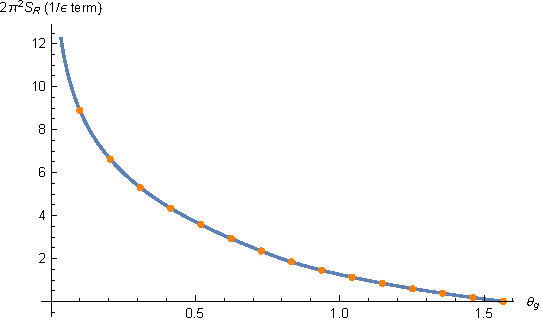
\includegraphics[width=0.75\columnwidth]{figures/full_non_divergent.pdf}
		\caption{\label{fig:non-divergent integral} Analytic (solid blue line) and numeric (orange dots) values of the $\epsilon^{-1}$ contribution to the soft function. Numerics are calculated from the integral of Eq.~\ref{eq:integral with divergence extracted}, and the analytic solution is that of Eq.~\ref{eq:analytic integral solution}.}
	\end{figure}
	The full soft function is therefore
	\begin{equation}\label{eq:full soft function}
	\boxed{
	\begin{aligned}
		S_R &= -\frac{2\pi\alpha_s C_F\mu^{2\epsilon}}{\pi^{5/2} \Gamma(\frac{1}{2} - \epsilon)}\qty(\frac{Q}{4})^{-2\epsilon} \frac{1}{\rho^{1 + 2\epsilon}} \\
			&\qquad\times \Bigg[\frac{1}{2\epsilon}\frac{\sqrt{\pi} \, \Gamma(\frac{1}{2} - \epsilon)}{\Gamma(1 - \epsilon)} - \qty[\pi - \arcsec(1 + \sec\theta_g)]\log\cot\frac{\theta_g}{2} \\
			&\qquad\qquad - \arcsec\qty(1 + \sec\theta_g) \log(2\cot\theta_g) \\
			&\qquad\qquad - \frac{i}{4}\qty[\Li_2\qty(-e^{-2i\arcsec\qty(1 + \sec\theta_g)}) - \Li_2\qty(-e^{2i\arcsec\qty(1 + \sec\theta_g)})] \\
			&\qquad\qquad+ \Theta\qty(\theta_g - \frac{\pi}{4})\Bigg[ \arccos\cot\theta_g \log(2\cot\theta_g) \\
			&\hspace{4.25cm}+ \frac{i}{4}\qty[\Li_2\qty(-e^{-2i\arccos\cot\theta_g}) - \Li_2\qty(-e^{2i\arccos\cot\theta_g})] \Bigg] + \cO(\epsilon) \Bigg].
	\end{aligned}
	}
	\end{equation}

\section{Second term}
	Now let us consider the second term of Eq.~\ref{eq:matrix element general}, which corresponds to emission off of the quark-gluon dipole. We have {\color{red}\textbf{[TODO: prefactor isn't quite right]}} \cite{catani_infrared_2000}
	\begin{equation}
		\abs{\cM_2}^2 = -\vb{T}_g \cdot \vb{T}_q \mu^{2\epsilon} \frac{n_q \cdot n_g}{(n_q \cdot k)(n_g \cdot k)} = -\vb{T}_g \cdot \vb{T}_q \mu^{2\epsilon} \frac{1 - \cos\theta_g}{k^+(n_g \cdot k)}.
	\end{equation}
	The phase space and grooming functions are all the same, so the contribution to compute is
	\begin{equation}\label{eq:soft integral II}
	\begin{aligned}
		S_R^{II}(\rho - \zcut) = -\vb{T}_g \cdot \vb{T}_q\mu^{2\epsilon} \int& \frac{d^d k}{(2\pi)^{d-1}} \, \delta\qty(k^2)\,\Theta(k^+)\,\Theta(k^- - k^+) \,\frac{1 - \cos\theta_g}{k^+(n_g \cdot k)} \\
		&\times \qty[\Theta(k\cdot n_g - k^+)\,\delta\qty(\rho - \frac{4k^+}{Q}) + \Theta(k^+ - k\cdot n_g)\,\delta\qty(\rho - \frac{4k\cdot n_g}{Q})] \\
		&\times \qty[1 - \Theta(k^+ - k^0 n_g \cdot n_q)\,\Theta(k \cdot n_g - k^0 n_g \cdot n_q)].
	\end{aligned}
	\end{equation}
	Under the coordinate choices described above, the matrix element becomes (from Eqs.~\ref{eq:kplus coordinates} and \ref{eq:k dot ng coordinates})
	\begin{equation}
		\abs{\cM_2}^2 \propto \frac{\qty(1 - \cos\theta_g)e^{\eta_k}}{k_\perp^2 \qty[\cosh\eta_k - \cos\phi_k \sin\theta_g - \sinh\eta_k \cos\theta_g]},
	\end{equation}
	so the full function to compute becomes
	\begin{equation}\label{eq:full integral 2}
	\boxed{
	\begin{aligned}
		S_R^{II}(\rho - \zcut) &= -\vb{T}_g \cdot \vb{T}_q\frac{\mu^{2\epsilon}\qty(1 - \cos\theta_g)}{4\pi^{5/2} \Gamma(\frac{1}{2} - \epsilon)}\int dk_\perp d\phi_k d\eta_k\, \sin^{-2\epsilon}\phi_k \, \Theta(k_\perp)\Theta(\eta_k) \\
		&\times\frac{e^{\eta_k}}{k_\perp^{1+2\epsilon} \qty[\cosh\eta_k - \cos\phi_k \sin\theta_g - \sinh\eta_k \cos\theta_g]} \\
		&\times \Bigg[ \Theta\qty(\sinh\eta_k - \cos\phi_k\cot\frac{\theta_g}{2})\,\delta\qty(\rho - \frac{4 k_\perp e^{-\eta_k}}{Q}) \\
			&\qquad+ \Theta\qty(\cos\phi_k\cot\frac{\theta_g}{2} - \sinh\eta_k)\, \delta\qty(\rho - \frac{4 k_\perp}{Q}\qty[\cosh\eta_k - \cos\phi_k\sin\theta_g - \sinh\eta_k\cos\theta_g])\Bigg] \\
			&\times \qty[1 - \Theta(\cos\theta_g - \tanh\eta_k)\,\Theta\qty(\cot\theta_g - e^{\eta_k}\cos\phi_k)].
	\end{aligned}
	}
	\end{equation}
	Integrating out $k_\perp$ leaves us with
	\begin{equation}
	\begin{aligned}
		S_R^{II} = -\vb{T}_g \cdot \vb{T}_q &\frac{\mu^{2\epsilon}\qty(1 - \cos\theta_g)}{4\pi^{5/2} \Gamma(\frac{1}{2} - \epsilon)} \qty(\frac{Q}{4})^{-2\epsilon} \frac{1}{\rho^{1+2\epsilon}} \int d\phi_k d\eta_k\, \sin^{-2\epsilon}\phi_k \, \Theta(\eta_k) \\
		&\times\frac{e^{\eta_k}}{\cosh\eta_k - \cos\phi_k \sin\theta_g - \sinh\eta_k \cos\theta_g} \\
		&\times \Bigg[ \Theta\qty(\sinh\eta_k - \cos\phi_k\cot\frac{\theta_g}{2})\,e^{-2\epsilon\eta_k} \\
			&\qquad+ \Theta\qty(\cos\phi_k\cot\frac{\theta_g}{2} - \sinh\eta_k)\, \qty(\frac{1}{\cosh\eta_k - \cos\phi_k\sin\theta_g - \sinh\eta_k\cos\theta_g})^{-2\epsilon}\Bigg] \\
		&\times \qty[1 - \Theta(\cos\theta_g - \tanh\eta_k)\,\Theta\qty(\cot\theta_g - e^{\eta_k}\cos\phi_k)].
	\end{aligned}
	\end{equation}
	Performing the same trick as in Eqs.~\ref{eq:theta expansion trick 1} and \ref{eq:theta expansion trick 2}, we then have
	\begin{equation}
	\begin{aligned}
		S_R^{II} = -\vb{T}_g \cdot \vb{T}_q &\frac{\mu^{2\epsilon}\qty(1 - \cos\theta_g)}{4\pi^{5/2} \Gamma(\frac{1}{2} - \epsilon)} \qty(\frac{Q}{4})^{-2\epsilon} \frac{1}{\rho^{1+2\epsilon}} \int d\phi_k d\eta_k\, \sin^{-2\epsilon}\phi_k \, \Theta(\eta_k) \\
		&\times\frac{e^{\eta_k - 2\epsilon\eta_k}}{\cosh\eta_k - \cos\phi_k \sin\theta_g - \sinh\eta_k \cos\theta_g} \\
		&\times \qty[1 - \Theta(\cos\theta_g - \tanh\eta_k)\,\Theta\qty(\cot\theta_g - e^{\eta_k}\cos\phi_k)] + \cO(\epsilon).
	\end{aligned}
	\end{equation}
	{\color{red}\textbf{[TODO: ask Andrew about this integral]}}

\section{Laplace transformation}
	For the rest of our analysis, it will be convenient to work in Laplace space. This is because Laplace transformation turns convolution into a simple product. Our factorization theorem involves a convolution of multiple functions, and a product is easier to work with. Luckily, the Laplace transformation of the soft function Eq.~\ref{eq:full soft function} in $\rho$ is quite straightforward. Transforming $\rho \to \nu$, we have
	\begin{equation}
		\cL\qty{\frac{1}{\rho^{1+2\epsilon}}} = \int_0^\infty \frac{d\rho}{\rho^{1+2\epsilon}} e^{-\rho\nu} = \nu^{2\epsilon} \Gamma(-2\epsilon).
	\end{equation}
	The Laplace-transformed soft function is therefore simply
	\begin{equation}
	\begin{aligned}
		\cL\qty{S_R} &= -\frac{2\pi\alpha_s C_F\mu^{2\epsilon}}{\pi^{5/2} \Gamma(\frac{1}{2} - \epsilon)}\qty(\frac{Q}{4})^{-2\epsilon} \nu^{2\epsilon} \Gamma(-2\epsilon) \\
			&\qquad\times \Bigg[\frac{1}{2\epsilon}\frac{\sqrt{\pi} \, \Gamma(\frac{1}{2} - \epsilon)}{\Gamma(1 - \epsilon)} - \qty[\pi - \arcsec(1 + \sec\theta_g)]\log\cot\frac{\theta_g}{2} \\
			&\qquad\qquad - \arcsec\qty(1 + \sec\theta_g) \log(2\cot\theta_g) \\
			&\qquad\qquad - \frac{i}{4}\qty[\Li_2\qty(-e^{-2i\arcsec\qty(1 + \sec\theta_g)}) - \Li_2\qty(-e^{2i\arcsec\qty(1 + \sec\theta_g)})] \\
			&\qquad\qquad+ \Theta\qty(\theta_g - \frac{\pi}{4})\Bigg[ \arccos\cot\theta_g \log(2\cot\theta_g) \\
			&\hspace{4cm}+ \frac{i}{4}\qty[\Li_2\qty(-e^{-2i\arccos\cot\theta_g}) - \Li_2\qty(-e^{2i\arccos\cot\theta_g})] \Bigg] + \cO(\epsilon) \Bigg].
	\end{aligned}
	\end{equation}

\subsection{Expansion}
	Now we can expand to partial $0$-th order in $\epsilon$. The prefactor becomes (after setting $\gamma_E \to 0$)
	\begin{equation}
	\begin{aligned}
		\frac{2\pi\alpha_s C_F\mu^{2\epsilon}}{\pi^{5/2} \Gamma(\frac{1}{2} - \epsilon)}\qty(\frac{Q}{4})^{-2\epsilon} \nu^{2\epsilon} \Gamma(-2\epsilon) = \frac{\alpha_s C_F}{\pi^2}\qty[-\frac{1}{\epsilon} + 2\log(\frac{Q}{2\nu}) - 2\log\mu - 2\epsilon\log(\frac{\mu\nu}{Q})\log(\frac{4\mu\nu}{Q})] + \cO(\epsilon).
	\end{aligned}
	\end{equation}
	Since
	\begin{equation}
		\log(\frac{\mu\nu}{Q})\log(\frac{4\mu\nu}{Q}) = \log^2\mu + \log\mu\log(\frac{4\nu^2}{Q^2}) + \log(\frac{\nu}{Q})\log(\frac{4\nu}{Q})
	\end{equation}
	and ultimately we only care about factors of $\log \mu$ to order $\epsilon^0$, we can then write
	\begin{equation}
		\frac{2\pi\alpha_s C_F\mu^{2\epsilon}}{\pi^{5/2} \Gamma(\frac{1}{2} - \epsilon)}\qty(\frac{Q}{4})^{-2\epsilon} \nu^{2\epsilon} \Gamma(-2\epsilon) = \frac{\alpha_s C_F}{\pi^2}\qty[-\frac{1}{\epsilon} + 2\log(\frac{Q}{2\nu}) - 2\log\mu - 2\epsilon\qty(\log^2\mu + \log\mu\log(\frac{4\nu^2}{Q^2}))] + \cO(\epsilon).
	\end{equation}
	We also have
	\begin{equation}
		\frac{1}{2\epsilon}\frac{\sqrt{\pi} \, \Gamma(\frac{1}{2} - \epsilon)}{\Gamma(1 - \epsilon)} = \frac{\pi}{2\epsilon} + \pi \log 2 + \cO(\epsilon).
	\end{equation}
	The soft function then becomes
	\begin{equation}\label{eq:transformed soft function partial order}
	\boxed{
	\begin{aligned}
		\cL\qty{S_R} &= -\frac{\alpha_s C_F}{\pi^2}\qty[-\frac{1}{\epsilon} + 2\log(\frac{Q}{2\nu}) - 2\log\mu - 2\epsilon\qty(\log^2\mu + \log\mu\log(\frac{4\nu^2}{Q^2}))] \\
			&\qquad\times \Bigg[\frac{\pi}{2\epsilon} + \pi \log 2 - \qty[\pi - \arcsec(1 + \sec\theta_g)]\log\cot\frac{\theta_g}{2} \\
			&\qquad\qquad - \arcsec\qty(1 + \sec\theta_g) \log(2\cot\theta_g) \\
			&\qquad\qquad - \frac{i}{4}\qty[\Li_2\qty(-e^{-2i\arcsec\qty(1 + \sec\theta_g)}) - \Li_2\qty(-e^{2i\arcsec\qty(1 + \sec\theta_g)})] \\
			&\qquad\qquad+ \Theta\qty(\theta_g - \frac{\pi}{4})\Bigg[ \arccos\cot\theta_g \log(2\cot\theta_g) \\
			&\hspace{3cm}+ \frac{i}{4}\qty[\Li_2\qty(-e^{-2i\arccos\cot\theta_g}) - \Li_2\qty(-e^{2i\arccos\cot\theta_g})] \Bigg] \Bigg] + \cO(\epsilon^0).
	\end{aligned}
	}
	\end{equation}
	Notice that the overall order of the expansion has been reduced because there are terms of order $\epsilon$ --- we just don't care about them because they do not come along with a $\log\mu$.


\section{Resummation}
\subsection{Strategy}
	We would like to renormalize the resolved soft function as in \cite{frye_factorization_2016}. We do this by demanding that the final total cross section be independent of $\mu$. The scale $\mu$, after all, was introduced solely to mathematically regulate divergences; it has no physical meaning.

	Suppose now that we have a cross section which is the product of two functions in Laplace space:
	\begin{equation}
		\sigma = F_1 F_2.
	\end{equation}
	Also suppose that $F_1$ and $F_2$ each have an anomalous dimension (i.e., the coefficient of the $1/\epsilon$ divergence in their Laurent expansion) of $\gamma_1$ and $\gamma_2$, respectively. It is a general result of QFT {\color{red}\textbf{[need to look into this more]}} that \cite{frye_factorization_2016}
	\begin{align}
		\frac{\partial F_1}{\partial \log \mu} &= \gamma_1 F_1 & \frac{\partial F_2}{\partial \log \mu} &= \gamma_1 F_2.
	\end{align}
	Then the product rule reveals that
	\begin{equation}
		\frac{\partial \sigma}{\partial \log \mu} = \frac{\partial F_1}{\partial \log \mu}F_2 + F_1 \frac{\partial F_2}{\partial \log \mu} = \qty(\gamma_1 + \gamma_2) F_1 F_2.
	\end{equation}
	Since we demand that $\partial \sigma /\partial \mu = 0$, it must be the case that the anomalous dimensions sum to zero,
	\begin{equation}
		\gamma_1 + \gamma_2 = 0.
	\end{equation}
	We can use this relationship to check the consistency of the factorization at the end.

	The renormalization scheme for now is to demand that
	\begin{equation}\label{eq:renormalization equation in mu}
		\frac{\partial F}{\partial \log\mu} = \gamma F
	\end{equation}
	for the anomalous dimension $\gamma$. Then if $\mu_1$ is the infrared scale of the $\mu$-logarithms, we can write the anomalous dimension as \cite{frye_factorization_2016}
	\begin{equation}
		\gamma = \Gamma_{F}(\alpha_s)\log\frac{\mu^2}{\mu_1^2} + \gamma_F(\alpha_s),
	\end{equation}
	where $\Gamma_F(\alpha_s)$ is the cusp anomalous dimension and $\gamma_F(\alpha_s)$ is the non-cusp anomalous dimension. These can be calculated order-by-order in $\alpha_s$ --- the non-cusp part is calculated as in previous sections, while the cusp part has a universal expansion up to a normalization \cite{frye_factorization_2016} {\color{red}\textbf{[is this right?]}}. Now we can convert between the renormalization scale $\mu$ and the strong coupling $\alpha_s$ using the $\beta$-function defined by
	\begin{equation}
		d\log\mu = \frac{d\alpha_s}{\beta(\alpha_s)}
	\end{equation}
	(notice the connections with the running of the strong coupling). Thus, the renormalization equation \ref{eq:renormalization equation in mu} becomes {\color{red}\textbf{[I think this is wrong but it doesn't matter\dots not using it right now anyway]}}
	\begin{equation}
		\beta(\alpha_s)\frac{\partial F}{\partial \alpha_s} = \qty[\Gamma_{F}(\alpha_s)\log\frac{\mu^2}{\mu_1^2} + \gamma_F(\alpha_s)]F(\mu).
	\end{equation}
	The solution to the differential equation is \cite{frye_factorization_2016}
	\begin{equation}\label{eq:renormalization solution}
	\begin{aligned}
		F(\mu) = F(\mu_0) \exp\Bigg[ 2\int_{\alpha_s(\mu_0)}^{\alpha_s(\mu)} \frac{d\alpha}{\beta(\alpha)}\Gamma_F(\alpha)\int_{\alpha_s(\mu_0)}^\alpha \frac{d\alpha'}{\beta(\alpha')} &+ \int_{\alpha_s(\mu_0)}^{\alpha_s(\mu)} \frac{d\alpha}{\beta(\alpha)}\gamma_F(\alpha) \\ 
			&+ \log\frac{\mu_0^2}{\mu_1^2}\int_{\alpha_s(\mu_0)}^{\alpha_s(\mu)} \frac{d\alpha}{\beta(\alpha)}\Gamma_F(\alpha) \Bigg]
	\end{aligned}
	\end{equation}
	where $\mu_0$ is an arbitrary reference scale.

	We can use this equation to evaluate the function to arbitrary accuracy, if we know the integrands to sufficiently high order. The cusp part of the anomalous dimension is, again, known and universal. The particular goal here is to identify the non-cusp contribution to the anomalous dimension.

\subsection{Anomalous dimension}
	The first step is to determine the anomalous dimension for the soft resolved function. Starting at Eq.~\ref{eq:transformed soft function partial order}, we have
	\begin{equation}
		\cL\qty{S_R} = -\frac{\alpha_s C_F}{\pi^2}\qty[-\frac{1}{\epsilon} - 2\log(\frac{2\mu\nu}{Q}) - 2\epsilon\qty(\log^2\mu + \log\mu \log(\frac{4\nu^2}{Q^2}))]\qty[\frac{\pi}{2\epsilon} + f(\theta_g)] + \cO(\epsilon^0)
	\end{equation}
	with
	\begin{equation}\label{eq:non-cusp f function}
	\begin{aligned}
		f(\theta_g) &= -\frac{1}{2\pi^3}\Bigg[\pi \log 2 - \qty[\pi - \arcsec(1 + \sec\theta_g)]\log\cot\frac{\theta_g}{2} - \arcsec\qty(1 + \sec\theta_g) \log(2\cot\theta_g) \\
			&\qquad\qquad - \frac{i}{4}\qty[\Li_2\qty(-e^{-2i\arcsec\qty(1 + \sec\theta_g)}) - \Li_2\qty(-e^{2i\arcsec\qty(1 + \sec\theta_g)})] \\
			&\qquad\qquad+ \Theta\qty(\theta_g - \frac{\pi}{4})\Bigg[ \arccos\cot\theta_g \log(2\cot\theta_g) \\
			&\hspace{5cm}+ \frac{i}{4}\qty[\Li_2\qty(-e^{-2i\arccos\cot\theta_g}) - \Li_2\qty(-e^{2i\arccos\cot\theta_g})] \Bigg]\Bigg].
	\end{aligned}
	\end{equation}
	Now, in general, the cusp anomalous dimension has expansion \cite{frye_factorization_2016}
	\begin{equation}
		\Gamma_{F}(\alpha_s) = d_F\Gamma_\cusp(\alpha_s) = d_F\sum_{n = 0}^\infty \Gamma_n \qty(\frac{\alpha_s}{4\pi})^{n+1}
	\end{equation}
	for some normalization $d_F$, and the non-cusp anomalous dimension has expansion
	\begin{equation}
		\gamma_F(\alpha_s) = \sum_{n = 0}^\infty \gamma_n \qty(\frac{\alpha_s}{4\pi})^{n+1}.
	\end{equation}
	We wish to determine the coefficients $\Gamma_n$ and $\gamma_n$. Expanding out the soft function, we have
	\begin{equation}
	\begin{aligned}
		\cL\qty{S_R} &= -\frac{\alpha_s C_F}{\pi^2}\qty[-\frac{\pi}{2\epsilon^2} - \frac{f(\theta_g)}{\epsilon} - \frac{\pi}{\epsilon}\log(\frac{2\mu \nu}{Q}) - \pi\qty(\log^2\mu + \log\mu\log(\frac{4\nu^2}{Q^2}))] + \cO(\epsilon^0) \\
		&= \frac{\alpha_s C_F}{4\pi}\qty[\frac{2}{\epsilon^2} + \frac{4f(\theta_g)}{\pi\epsilon} + \frac{4}{\epsilon}\log(\frac{2\mu \nu}{Q}) + \frac{1}{4}\qty(\log^2\mu + \log\mu\log(\frac{4\nu^2}{Q^2}))] + \cO(\epsilon^0).
	\end{aligned}
	\end{equation}
	The anomalous dimension is the coefficient of $1/\epsilon$:
	\begin{equation}
		\gamma_{S_R} = \frac{\alpha_s C_F}{4\pi}\qty[\frac{4f(\theta_g)}{\pi} + 2\log(\frac{4\mu^2\nu^2}{Q^2})].
	\end{equation}
	Notice that this takes the form {\color{red}\textbf{[is this supposed to happen? or is it weird to have a $\log \mu$ with a $1/\epsilon$?]}}
	\begin{equation}
		\gamma = \Gamma_{S_R}(\alpha_s)\log\frac{\mu^2}{\mu_1^2} + \gamma_{S_R}(\alpha_s)
	\end{equation}
	with infrared scale
	\begin{equation}
		\mu_1 = \frac{Q}{2\nu},
	\end{equation}
	cusp anomalous dimension
	\begin{equation}\label{eq:soft cusp anomalous dimension}
		\Gamma_{S_R}(\alpha_s) = 2C_F \qty(\frac{\alpha_s}{4\pi}),
	\end{equation}
	and non-cusp anomalous dimension
	\begin{equation}
		\gamma_{S_R}(\alpha_s) = \frac{4C_F}{\pi}f(\theta_g)\qty(\frac{\alpha_s}{4\pi}).
	\end{equation}
	Therefore, to one-loop accuracy {\color{red}\textbf{[correct terminology?]}}, the cusp anomalous dimension is
	\begin{equation}
		\Gamma_{S_R} = \frac{C_F}{2} \Gamma_\cusp
	\end{equation}
	where \cite{frye_factorization_2016}
	\begin{equation}
		\Gamma_\cusp = 4\qty(\frac{\alpha_s}{4\pi}) + \cO(\alpha_s^2)
	\end{equation}
	{\color{red}\textbf{[is this right?]}}. The non-cusp anomalous dimension has a one-loop coefficient
	\begin{equation}\label{eq:non-cusp anomalous dimension}
		\boxed{\gamma_0 = \frac{4C_F}{\pi}f(\theta_g).}
	\end{equation}

\subsection{Evaluation}
	Now that we have $\gamma_0$ in hand, we wish to evaluate Eq.~\ref{eq:renormalization solution}. 
	% To one-loop order, this reads
	% \begin{equation}
	% \begin{aligned}
	% 	F(\mu) = F(\mu_0) \exp\Bigg[ 2\int_{\alpha_s(\mu_0)}^{\alpha_s(\mu)} \frac{d\alpha}{\beta(\alpha)}\Gamma_F \frac{\alpha}{4\pi} \int_{\alpha_s(\mu_0)}^\alpha \frac{d\alpha'}{\beta(\alpha')} &+ \int_{\alpha_s(\mu_0)}^{\alpha_s(\mu)}\frac{d\alpha}{\beta(\alpha)}\gamma_0 \frac{\alpha}{4\pi} \\
	% 		&+ \log\frac{\mu_0^2}{\mu_1^2} \int_{\alpha_s(\mu_0)}^{\alpha_s(\mu)} \frac{d\alpha}{\beta(\alpha)} \Gamma_0 \frac{\alpha}{4\pi }\Bigg].
	% \end{aligned}
	% \end{equation}
	The $\beta$-function can be written as a power series
	\begin{equation}
		\beta(\alpha_s) = \mu\frac{\partial \alpha_s}{\partial\mu} = -2\alpha_s \sum_{n = 0}^\infty \beta_n \qty(\frac{\alpha_s}{4\pi})^{n+1}
	\end{equation}
	where the coefficients are known \cite{frye_factorization_2016}
	\begin{equation}\label{eq:beta coefficients}
	\begin{aligned}
		\beta_0 &= \frac{11}{3}C_A - \frac{4}{3}T_R n_f \\
		\beta_1 &= \frac{34}{3}C_A^2 - 4T_Rn_f\qty(C_F + \frac{5}{3}C_A).
	\end{aligned}
	\end{equation}
	{\color{red}\textbf{[TODO: figure out what $T_R$ and $n_f$ are]}}. The cusp anomalous dimension coefficients are also known to one-loop order:
	\begin{equation}\label{eq:cusp coefficients}
	\begin{aligned}
		\Gamma_0 &= 4 \\
		\Gamma_1 &= 4C_A\qty(\frac{67}{9} - \frac{\pi^2}{3}) - \frac{80}{9}T_R n_f.
	\end{aligned}
	\end{equation}
	Now we can perform each integral. With $\gamma_0$, we ought to be able to push to NLL order, so we want the exponent to have power $\alpha_s^0$. The first exponentiated integral is
	\begin{equation}
		\int_{\alpha_s(\mu_0)}^{\alpha_s(\mu)} \frac{d\alpha}{\beta(\alpha)}\Gamma_F(\alpha)\int_{\alpha_s(\mu_0)}^\alpha \frac{d\alpha'}{\beta(\alpha')} = A + \cO(\alpha_s).
	\end{equation}
	If we want this integral to order $\alpha_s^0$, then we need its integrand to order $\alpha_s^{-1}$:
	\begin{equation}
		\frac{\Gamma_F(\alpha)}{\beta(\alpha)}\int_{\alpha_s(\mu_0)}^\alpha \frac{d\alpha'}{\beta(\alpha')} = B + \cO(\alpha^0).
	\end{equation}
	Now, $1/\beta(\alpha_s)$ has an order-2 pole a at $\alpha_s = 0$, so we can divide this integral into two Laurent series
	\begin{equation}
	\begin{aligned}
		\frac{\Gamma_F(\alpha)}{\beta(\alpha)} &= \frac{A_1}{\alpha} + A_2 \\
		\int_{\alpha_s(\mu_0)}^\alpha \frac{d\alpha'}{\beta(\alpha')} &= \frac{B_1}{\alpha} + B_2 \\
		\frac{\Gamma_F(\alpha)}{\beta(\alpha)}\int_{\alpha_s(\mu_0)}^\alpha \frac{d\alpha'}{\beta(\alpha')} &= \frac{A_1B_1}{\alpha^2} + \frac{A_1 B_2 + A_2 B_1}{\alpha} + \cO(\alpha^0).
	\end{aligned}
	\end{equation}
	Now to get the expression in the second line, we need to know $1/\beta(\alpha')$ to order $(\alpha')^{-1}$. Thus,
	\begin{equation}
	\begin{aligned}
		\int_{\alpha_s(\mu_0)}^\alpha \frac{d\alpha'}{\beta(\alpha')} &= -\frac{1}{2\beta_0}\int_{\alpha_s(\mu_0)}^\alpha d\alpha' \qty[\frac{4\pi}{(\alpha')^2} - \frac{\beta_1}{\beta_0 \alpha'} + \cO((\alpha')^0] \\
		&= \frac{1}{2\beta_0}\eval{\qty[\frac{4\pi}{\alpha'} + \frac{\beta_1}{\beta_2}\log\alpha']}_{\alpha' = \alpha_s(\mu_0)}^\alpha + \cO(\alpha) \\
		&= \frac{1}{2\beta_0}\qty[4\pi\qty(\frac{1}{\alpha} - \frac{1}{\alpha_s(\mu_0)}) + \frac{\beta_1}{\beta_0}\log\frac{\alpha}{\alpha_s(\mu_0)}] + \cO(\alpha).
	\end{aligned}
	\end{equation}
	If $\Gamma_F = d_F \Gamma_\cusp$, the integrand of interest then becomes
	\begin{equation}
	\begin{aligned}
		\frac{\Gamma_F(\alpha)}{\beta(\alpha)}\int_{\alpha_s(\mu_0)}^\alpha \frac{d\alpha'}{\beta(\alpha')} &= \frac{d_F}{4\beta_0^2}\qty[-\frac{\Gamma_0}{\alpha} + \frac{\beta_1 \Gamma_0 - \beta_0 \Gamma_1}{4\pi\beta_0}]\qty[4\pi\qty(\frac{1}{\alpha} - \frac{1}{\alpha_s(\mu_0)}) + \frac{\beta_1}{\beta_0}\log\frac{\alpha}{\alpha_s(\mu_0)}] + \cO(\alpha^0) \\
		&= \frac{d_F}{4\beta_0^2}\qty[\frac{4\pi \Gamma_0}{\alpha}\qty(\frac{1}{\alpha_s(\mu_0)} - \frac{1}{\alpha}) - \frac{\Gamma_0 \beta_1}{\beta_0 \alpha}\log\frac{\alpha}{\alpha_s(\mu_0)} + \frac{\beta_1 \Gamma_0 - \beta_0 \Gamma_1}{\beta_0 \alpha}] + \cO(\alpha^0) \\
		&= \frac{d_F\Gamma_0}{4\beta_0^2}\qty[-\frac{4\pi}{\alpha^2} + \frac{1}{\alpha}\qty(\frac{\beta_1\Gamma_0 - \beta_0 \Gamma_1}{\beta_0\Gamma_0} + \frac{4\pi}{\alpha_s(\mu_0)} - \frac{\beta_1}{\beta_0}\log\frac{\alpha}{\alpha_s(\mu_0)})] + \cO(\alpha^0).
	\end{aligned}
	\end{equation}
	This is now straightforward to integrate:
	\begin{equation}
	\begin{aligned}
		\int_{\alpha_s(\mu_0)}^{\alpha_s(\mu)} \frac{d\alpha}{\beta(\alpha)}&\Gamma_F(\alpha)\int_{\alpha_s(\mu_0)}^\alpha \frac{d\alpha'}{\beta(\alpha')} \\
		&= \frac{d_F\Gamma_0}{4\beta_0^2}\Bigg[ \frac{4\pi}{\alpha} + \log\alpha \qty(\frac{\beta_1\Gamma_0 - \beta_0 \Gamma_1}{\beta_0\Gamma_0} + \frac{4\pi}{\alpha_s(\mu_0)}) + \frac{\beta_1}{2\beta_0}\log^2\qty(\frac{\alpha}{\alpha_s(\mu_0)}) \eval{\Bigg]}_{\alpha = \alpha_s(\mu_0)}^{\alpha_s(\mu)} + \cO(\alpha_s) \\
		&= \frac{d_F\Gamma_0}{4\beta_0^2}\Bigg[4\pi\qty(\frac{1}{\alpha_s(\mu)} - \frac{1}{\alpha_s(\mu_0)}) + \log\frac{\alpha_s(\mu)}{\alpha_s(\mu_0)}\qty(\frac{\beta_1\Gamma_0 - \beta_0 \Gamma_1}{\beta_0\Gamma_0} + \frac{4\pi}{\alpha_s(\mu_0)}) \\
			&\qquad\qquad+ \frac{\beta_1}{2\beta_0}\log^2\qty(\frac{\alpha_s(\mu)}{\alpha_s(\mu_0)})\Bigg] + \cO(\alpha_s).
	\end{aligned}
	\end{equation}
	If we let
	\begin{equation}
		r = \frac{\alpha_s(\mu)}{\alpha_s(\mu_0)},
	\end{equation}
	we end up with
	\begin{equation}\label{eq:first exponentiated integral}
	\begin{aligned}
		\int_{\alpha_s(\mu_0)}^{\alpha_s(\mu)} \frac{d\alpha}{\beta(\alpha)}&\Gamma_F(\alpha)\int_{\alpha_s(\mu_0)}^\alpha \frac{d\alpha'}{\beta(\alpha')} \\
		&= \frac{d_F\Gamma_0}{4\beta_0^2}\Bigg[\frac{4\pi}{\alpha_s(\mu_0)}\qty(\log r + \frac{1}{r} - 1) + \log r \qty(\frac{\beta_1}{\beta_0} - \frac{\Gamma_1}{\Gamma_0}) + \frac{\beta_1}{2\beta_0}\log^2 r \Bigg] + \cO(\alpha_s).
	\end{aligned}
	\end{equation}

	The second exponentiated integral is
	\begin{equation}
		\int_{\alpha_s(\mu_0)}^{\alpha_s(\mu)} \frac{d\alpha}{\beta(\alpha)}\gamma_F(\alpha).
	\end{equation}
	If we want to know this integral to order $\alpha_s^0$, we need its integrand to order $\alpha_s^{-1}$:
	\begin{equation}
		\frac{\gamma_F(\alpha)}{\beta(\alpha)} = -\frac{\gamma_0}{2\beta_0\alpha} + \cO(\alpha^0).
	\end{equation}
	Hence,
	\begin{equation}\label{eq:second exponentiated integral}
		\int_{\alpha_s(\mu_0)}^{\alpha_s(\mu)} \frac{d\alpha}{\beta(\alpha)}\gamma_F(\alpha) = -\frac{\gamma_0}{2\beta_0}\log\frac{\alpha_s(\mu)}{\alpha_s(\mu_0)} + \cO(\alpha_s) = -\frac{\gamma_0}{2\beta_0}\log r + \cO(\alpha_s)
	\end{equation}
	The fully exponential term of Eq.~\ref{eq:renormalization solution} is then the sum of Eqs.~\ref{eq:first exponentiated integral} and \ref{eq:second exponentiated integral}.
	\begin{equation}\label{eq:exponentiated kernel}
	\begin{aligned}
		K_F(\mu, \mu_0) &\equiv 2\int_{\alpha_s(\mu_0)}^{\alpha_s(\mu)} \frac{d\alpha}{\beta(\alpha)}\Gamma_F(\alpha)\int_{\alpha_s(\mu_0)}^\alpha \frac{d\alpha'}{\beta(\alpha')} + \int_{\alpha_s(\mu_0)}^{\alpha_s(\mu)} \frac{d\alpha}{\beta(\alpha)}\gamma_F(\alpha) \\
		&= \frac{d_F\Gamma_0}{2\beta_0^2}\Bigg[\frac{4\pi}{\alpha_s(\mu_0)}\qty(\log r + \frac{1}{r} - 1) + \log r \qty(\frac{\beta_1}{\beta_0} - \frac{\Gamma_1}{\Gamma_0}) + \frac{\beta_1}{2\beta_0}\log^2 r \Bigg] - \frac{\gamma_0}{2\beta_0}\log r + \cO(\alpha_s).
	\end{aligned}
	\end{equation}

	The final integral of Eq.~\ref{eq:renormalization solution} is
	\begin{equation}\label{eq:third exponentiated integral}
	\begin{aligned}
		\omega(\mu, \mu_0) &\equiv \int_{\alpha_s(\mu_0)}^{\alpha_s(\mu)} \frac{d\alpha}{\beta(\alpha)}\Gamma_F(\alpha) \\
		&= \frac{d_F}{2\beta_0}\int_{\alpha_s(\mu_0)}^{\alpha_s(\mu)} d\alpha \qty[-\frac{\Gamma_0}{\alpha} + \frac{\beta_1\Gamma_0 - \beta_0 \Gamma_1}{4\pi \beta_0} + \cO(\alpha)] \\
		&= \frac{d_F \Gamma_0}{2\beta_0}\qty[\log \frac{1}{r} + \frac{\alpha_s(\mu_0)}{4\pi}(r - 1)\qty(\frac{\beta_1}{\beta_0} - \frac{\Gamma_1}{\Gamma_0})] + \cO(\alpha_s^2).
	\end{aligned}
	\end{equation}
	{\color{red}\textbf{[I'm following the Frye paper in going to order $\alpha_s$ here, but why?]}}. Then combining Eqs.~\ref{eq:renormalization solution}, \ref{eq:exponentiated kernel}, and \ref{eq:third exponentiated integral}, we have
	\begin{equation}
		\boxed{F(\mu) = F(\mu_0) e^{K(\mu, \mu_0)} \qty(\frac{\mu_0^2}{\mu_1^2})^{\omega(\mu, \mu_0)}}
	\end{equation}
	for some reference scale $\mu$, $\beta_i$ and $\Gamma_i$ defined in Eqs.~\ref{eq:beta coefficients} and \ref{eq:cusp coefficients}, respectively, and
	\begin{equation}
		\mu_1 = \frac{Q}{2\nu}.
	\end{equation}
	To be explicit about the resolved soft function, we have
	\begin{equation}\label{eq:resummed soft function laplace}
		\cL\qty{S_R(\nu, \mu)} = \cL\qty{S_R(\nu, \mu_0)} e^{K_{S_R}(\mu, \mu_0)} \qty(\frac{4 \mu_0^2}{Q^2}\nu^2)^{\omega_{S_R}(\mu, \mu_0)}
	\end{equation}
	{\color{red}\textbf{[how to calculate $\cL\qty{S_R(\mu_0)}$?]}}. From Eqs.~\ref{eq:soft cusp anomalous dimension} and \ref{eq:cusp coefficients}, we see that
	\begin{equation}
		\Gamma_{S_R}(\alpha) = 2C_F\qty(\frac{\alpha_s}{4\pi}) + \cO(\alpha_s^2) = 4d_{S_R} \qty(\frac{\alpha_s}{4\pi}) + \cO(\alpha_s^2),
	\end{equation}
	so $d_{S_R} = C_F/2$. The exponentiated kernel $K_{S_R}$ is then, from Eqs.~\ref{eq:non-cusp anomalous dimension} and \ref{eq:exponentiated kernel},
	\begin{equation}
	\begin{aligned}
		K_{S_R}(\mu, \mu_0) &= \frac{C_F\Gamma_0}{4\beta_0^2}\Bigg[\frac{4\pi}{\alpha_s(\mu_0)}\qty(\log r + \frac{1}{r} - 1) + \log r \qty(\frac{\beta_1}{\beta_0} - \frac{\Gamma_1}{\Gamma_0}) + \frac{\beta_1}{2\beta_0}\log^2 r \Bigg] \\
		&\qquad\qquad - \frac{2C_F}{\pi \beta_0}f(\theta_g)\log r + \cO(\alpha_s)
	\end{aligned}
	\end{equation}
	with $f(\theta_g)$ defined in Eq.~\ref{eq:non-cusp f function}. The exponent $\omega_{S_R}$ is simply
	\begin{equation}
		\omega_{S_R}(\mu, \mu_0) = \frac{C_F \Gamma_0}{4\beta_0}\qty[\log \frac{1}{r} + \frac{\alpha_s(\mu_0)}{4\pi}(r - 1)\qty(\frac{\beta_1}{\beta_0} - \frac{\Gamma_1}{\Gamma_0})] + \cO(\alpha_s^2).
	\end{equation}

\section{Inverse Laplace transform}
	Because the soft function $\cL\qty{S_R(\mu)}$ has explicit dependence on the Laplace-transformed mass $\nu$, its inverse transformation is nontrivial. Looking at Eq.~\ref{eq:resummed soft function laplace}, because logarithms in the function $\cL\qty{S_R(\nu, \mu_0)}$ have the same argument as the term raised to the $\omega_{S_R}$ power,
	\begin{equation}
		\frac{4\mu_0^2}{Q^2}\nu^2,
	\end{equation}
	we can use the relationship \cite{frye_factorization_2016,becher_factorization_2007}
	\begin{equation}
		\frac{\partial^n}{\partial q^n}\nu^q = \nu^q \log^n \nu
	\end{equation}
	to replace logarithms in the low-scale function $\cL\qty{S_R}$ with derivatives with respect to the exponentiated function $\omega_{S_R}(\mu, \mu_0)$. {\color{red}\textbf{[I don't fully understand this step yet]}}. Let
	\begin{equation}
		S_R(L \to \partial_{\omega_{S_R}})
	\end{equation}
	represent this transformation. Then we can re-write the soft resolved function as
	\begin{equation}
		\cL{S_R} = e^{K_{S_R}(\mu, \mu_0)}S_R(L \to \partial_{\omega_{S_R}}) \qty[\frac{4\mu_0^2}{Q^2}\nu^2]^{\omega_{S_R}(\mu, \mu_0)}.
	\end{equation}
	Now, the Laplace transform commutes with derivatives, so we can use the relation \cite{frye_factorization_2016}
	\begin{equation}
		\cL^{-1}\qty{\nu^q} = \frac{\rho^{-q-1}}{\Gamma(-q)}
	\end{equation}
	to find
	\begin{equation}
		\boxed{S_R(\rho, \mu) = e^{K_{S_R}(\mu, \mu_0)}S_R(L \to \partial_{\omega_{S_R}}) \qty[\frac{4\mu_0^2}{Q^2}\frac{1}{\rho^2}]^{\omega_{S_R}(\mu, \mu_0)} \frac{1}{\rho} \qty\big[\Gamma\qty(-2\omega_{S_R}(\mu, \mu_0))]^{-1}.}
	\end{equation}


% \subsection{Execution}
% 	The first step will be to take the $\log\mu$ derivative. Let us suggestively define
% 	\begin{equation}
% 	\begin{aligned}
% 		\gamma_{\nc} &= -\frac{1}{2\pi^3}\Bigg[\pi \log 2 - \qty[\pi - \arcsec(1 + \sec\theta_g)]\log\cot\frac{\theta_g}{2} - \arcsec\qty(1 + \sec\theta_g) \log(2\cot\theta_g) \\
% 			&\qquad\qquad - \frac{i}{4}\qty[\Li_2\qty(-e^{-2i\arcsec\qty(1 + \sec\theta_g)}) - \Li_2\qty(-e^{2i\arcsec\qty(1 + \sec\theta_g)})] \\
% 			&\qquad\qquad+ \Theta\qty(\theta_g - \frac{\pi}{4})\Bigg[ \arccos\cot\theta_g \log(2\cot\theta_g) \\
% 			&\hspace{5cm}+ \frac{i}{4}\qty[\Li_2\qty(-e^{-2i\arccos\cot\theta_g}) - \Li_2\qty(-e^{2i\arccos\cot\theta_g})] \Bigg]\Bigg],
% 	\end{aligned}
% 	\end{equation}
% 	so that the transformed soft function is
% 	\begin{equation}
% 	\begin{aligned}
% 		\cL\qty{S_R} &= \frac{1}{4\pi^3}\qty[-\frac{1}{\epsilon} + 2\log(\frac{Q}{2\nu}) - 2\log\mu - 2\epsilon\qty(\log^2\mu + \log\mu\log(\frac{4\nu^2}{Q^2}))] \qty[\frac{\pi}{2\epsilon} - 2\pi^3\gamma_{\nc}] + \cO(\epsilon^0) \\
% 		&= -\frac{1}{8\pi^2\epsilon^2} + \frac{1}{4\pi^2\epsilon}\qty[\log(\frac{Q}{2\nu}) - \log\mu] \\
% 			&\qquad\qquad- \gamma_{\nc}\qty(\log(\frac{Q}{2\nu}) - \log\mu) - \frac{1}{4\pi^2} \qty[\log^2\mu + \log\mu\log(\frac{4\nu^2}{Q^2})] + \cO(\epsilon^0).
% 	\end{aligned}
% 	\end{equation}
% 	We can go ahead and drop the pole at $\epsilon = 0$, since the divergences must cancel in the end anyway {\color{red}\textbf{[is this the right justification?]}}. We are left with
% 	\begin{equation}\label{eq:transformed soft dropped poles}
% 	\begin{aligned}
% 		\overline{\cL\qty{S_R}} &= - \gamma_{\nc}\qty(\log(\frac{Q}{2\nu}) - \log\mu) - \frac{1}{4\pi^2} \qty[\log^2\mu + \log\mu\log(\frac{4\nu^2}{Q^2})] + \cO(\epsilon^0) \\
% 		&= \gamma_\nc \log(\frac{2\mu\nu}{Q}) - \frac{1}{4\pi^2} \qty[\log^2\mu + \log\mu\log(\frac{4\nu^2}{Q^2})] + \cO(\epsilon^0).
% 	\end{aligned}
% 	\end{equation}
% 	Now taking the derivative with respect to $\log \mu$ is straightforward:
% 	\begin{equation}
% 	\begin{aligned}
% 		\frac{\partial \overline{\cL\qty{S_R}}}{\partial \log \mu} &= \gamma_\nc - \frac{1}{4\pi^2}\log(\frac{4\mu^2\nu^2}{Q^2}) + \cO(\epsilon^1).
% 	\end{aligned}
% 	\end{equation}
% 	Notice that this represents the full derivative to order $\epsilon^0$: any terms of order $\epsilon^0$ not represented in Eq.~\ref{eq:transformed soft dropped poles} are not associated with $\log \mu$. Then setting $\epsilon = 0$, we are left with
% 	\begin{equation}
% 		\frac{\partial \overline{\cL\qty{S_R}}}{\partial \log \mu} = \gamma_\nc - \frac{1}{2\pi^2}\log(\frac{2\mu\nu}{Q}).
% 	\end{equation}
% 	{\color{red}\textbf{[this does not appear to follow the renormalization equation\dots is it because the $S_R$ calculated up to here is not the function in the renormalization equation? Cf \cite{bell_automated_2015} section 5]}}


\bibliographystyle{unsrt}
\bibliography{jet_substructure}

\end{document}